\section{Cara Insert Database Mysql}

	\subsection{Database Mysql}}
	Basis data merupakan istilah yang mengacu kepada kumpulan data yang saling berhubungan satu sama lain, dan perangkat lunak harus mengacu pada sistem manajemen basis data DBMS. Jika konteksnya jelas, banyak administrator dan programer menggunakan istilah basis data untuk kedua makna, dan juga  merupakan sekumpulan data yang membentuk file yang saling berhubungan dengan format tertentu untuk membentuk data atau informasi baru. Atau database adalah kumpulan data yang saling berhubungan satu sama lain yang diatur berdasarkan skema atau struktur tertentu. Di komputer, basis data disimpan di perangkat penyimpanan perangkat keras, dan dengan perangkat lunak tertentu yang dimanipulasi oleh minat atau minat tertentu. 
	Hubungan atau hubungan data biasanya ditunjukkan oleh kunci dari setiap file. MySQL adalah sistem manajemen basis data perangkat lunak atau perangkat lunak SQL atau DBMS Multithread dan multi user. mysql sebenarnya merupakan turunan dari salah satu konsep utama dalam database untuk seleksi atau seleksi dan entri data yang memungkinkan operasi data dilakukan dengan mudah dan otomatis. 
	Michael Widenius merupakan seseorang yang menciptakan mysql pada tahun 1979, seorang programmer komputer swedia yang mengembangkan sistem database sederhana yang disebut unireg yang menggunakan koneksi mesin database isam tingkat rendah dengan pengindeksan. mysql adalah salah satu jenis server basis data yang paling populer.mysql menggunakan bahasa sql untuk mengakses database-nya. lisensi mysql adalah lisensi foss exception dan ada juga versi komersial. 
	Mysql tag adalah database sumber terbuka paling populer di dunia, dan sebenarnya merupakan turunan dari salah satu konsep utama dalam database yang sudah ada di sql. konsep operasi pada database terutama sql adalah untuk menseleksi atau seleksi dan entri data yang memungkinkan pengoperasian data dilakukan secara otomatis dengan mudah. 
	
	\subsection{Cara Penulisan Dasar Query INSERT}
	
	jika kita mengutip dari manual resmi MySQL sendiri, penulisan dasar perintah INSERT adalah seperti dibawah ini :
	
	\begin{verbatim}
		INSERT [LOW_PRIORITY | DELAYED | HIGH_PRIORITY] [IGNORE]
		[INTO] tbl_name [(col_name,...)]
		{VALUES | VALUE} ({expr | DEFAULT},...),(...),...
		[ ON DUPLICATE KEY UPDATE
		col_name=expr
		[, col_name=expr] ... ]
	\end{verbatim}
	
	\subsection{Cara Penggunaan Query INSERT...VALUES}
	Disini kita akan membahas perintah INSERT yang paling sederhana, yakni:
	
	\begin{verbatim}
		INSERT INTO nama_table VALUES (nilai_kolom1, nilai_kolom2,...);
	\end{verbatim}
	
	nama_table merupakan nama tabel yang akan kita input, dan nilai_kolom1 merupakan nilai yang akan kita imputkan ke dalam tabel tersebut, dan juga seterusnya untuk nilai kolom. Di nilai kolom haris berada dalam tanda kurung dan dipisah oleh tanda koma.
	
	Gambar dibawah adalah contoh memasukkan sebaris data :
	
	\begin{figure}[ht]
			\centerline{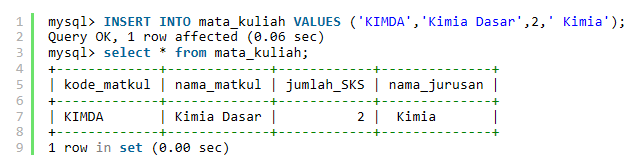
\includegraphics[width=0.5\textwidth]{figures/insert.png}}
			\caption{Insert}
			\label{insert}
			\end{figure}
			
	Kita juga bisa langsung memasukkan dua baris data ataupun lebih secara langsung hanya dengan satu perintah query INSERT, kita hanya butuh untuk memasukkan data di baris selanjutnya di belakang perintah, dengan bentuk seperti ini :
	
	\begin{verbatim}
		INSERT INTO nama_table VALUES (nilai_kolom1a, nilai_kolom2a,...), 
		(nilai_kolom1b, nilai_kolom2b,...);
	\end{verbatim}
	
	Gambar dibawah ini adalah contoh penambahan data dua baris sekaligus :
	
	\begin{figure}[ht]
			\centerline{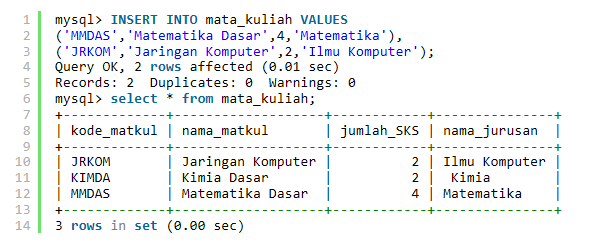
\includegraphics[width=0.5\textwidth]{figures/insert2.png}}
			\caption{Insert Dua Data}
			\label{insert2}
			\end{figure}
	
	command INSERT..VALUES diatas bagus digunakan apabila kita tau urutan - urutan kolom yang ada dalam tabel tersebut, kita diharuskan untuk menafsirkan urutan kolom yang ingin kita isi dengan cara menuliskan query INSERT..VALUES.
	
	\subsection{Cara Penggunaan Query INSERT(nama_kolom)...VALUES}
	Apabila kita berada di dalam situasi dimana kita tidak mengetahui urutan kolom yang akan kita isi, ataupun hanya ingin mengisi sebagian saja. Kita dapat menggunakan perintah seperti dibawah ini :
		\begin{verbatim}
			INSERT INTO nama_table (kolom1,kolom2,...) VALUES (nilai_kolom1,nilai_kolom2,...);
		\end{verbatim}
		
	Gambar dibawah ini adalah contoh dari perintah diatas :
	
		\begin{figure}[ht]
			\centerline{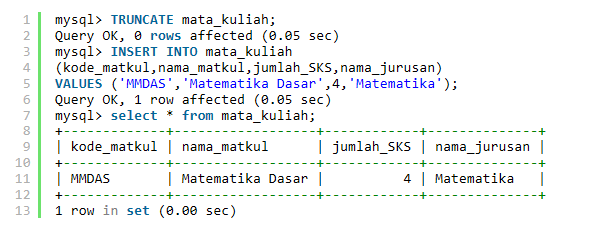
\includegraphics[width=0.5\textwidth]{figures/insert3.png}}
			\caption{Insert Tanpa Urutan}
			\label{insert3}
			\end{figure}
			
	command TRUNCATE diatas hanya untuk mengosongkan tabel diatas saja, jika tidak ingin mengosongkannya terlebih dahulu, kalian bisa mengabaikan command ini.
	
	Jika urutan kolom kita acak pun, tidak akan menjadi masalah asalkan perintah yang diinput tetap sesuai dengan urutan kolom tersebut, seperti gambar dibawah ini :
	
		\begin{figure}[ht]
			\centerline{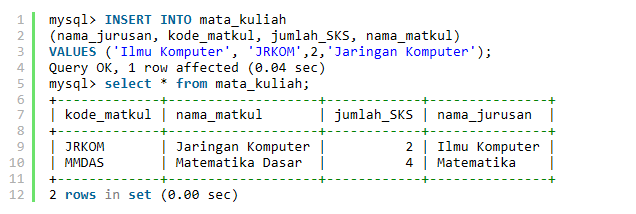
\includegraphics[width=0.5\textwidth]{figures/insert4.png}}
			\caption{Insert Kolom Acak}
			\label{insert4}
			\end{figure}
	
	Di dalam query saat pembuatan table mata_kuliah, kolom jumlah_SKS ditafsirkan memiliki nilai default 2, ajdi jika kolom ini tidak diisi pun , akan tetap menggunakan nilai defaultnya yaitu 2.
	
		\begin{figure}[ht]
			\centerline{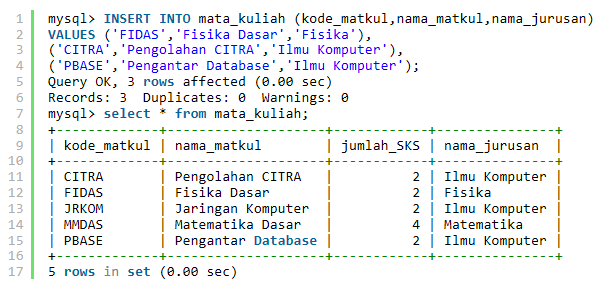
\includegraphics[width=0.5\textwidth]{figures/insert5.png}}
			\caption{Insert Tiga Kolom}
			\label{insert5}
			\end{figure}
			
	Pada gambar diatas hanya diisikan 3 kolom, tanpa memasukkan kolom jumlah_sks, tetapi karna kolom tersebut susah mempunyai nilai default 2, jadi akan tetap terisi.